\section{Data Collection}

\subsection{Participants}
The height females and the twelve males participants had from 18 to 30 years old (23 median and average years of age). The 20 subject were screened for correct visual acuity (no errors on 20/30 lines) and color vision using Snellen and Ishiara charts respectively. They all provided written consents forms. Before each experiment, oral instruction were provided to the participants to explain their tasks. Additionally, a training session was organized to allow participants to familiarize with the assessment procedure. The content shown in the training session was selected by experts viewers in order to include examples of all evaluated aspects.

\subsection{Audio-visual stimuli}
Video stimuli are coming from nine video sequences extracted from four open source movies published by the Blender Foundation (Big buck bunny, Elephant dream, Sintel and Tears of Steel)\footnote{$http://media.xiph.org/$}. A supplementary sequence content was chosen for the training session.
\\The one minutes selected video contents have the highest audio, spatial end temporal energy and are related to the scene cuts.
The twenty seven video stimuli shown during an experiment are the combination of the nine video content with the three levels of immersiveness described below.
\\Low, middle and high immersiveness level were defined respectively thanks to the audio sound system, the video quality\textbackslash level of compression and the resolution.
The table \ref{IL} illustrates the previous comment.

\begin{table}[h]
\begin{tabular}{ |c || c | c | c | }
   \hline	
   Immersive senario 	& Low 			& Middle 		& High \\
   \hline	
   Audio 				& No Audio 		& Stereo		& Surround \\
   Quality (QP) 		& 36 			& 20			& 20 \\
   Resolution			& SD			& HD			& UHD\\
   \hline	
 \end{tabular}
 \caption{immersiveness levels}
 \label{IL}
 \end{table}

The video stimuli order could impact the data and so the results. Thus the sessions are built to allow this study : The first session will display the video stimuli from the lowest immersiveness level stimuli to the ones with the highest level. The second session order is middle immersiveness level stimuli, followed by the low immersiveness level stimuli and then the high immersiveness level stimuli. The last session will display the video stimuli from the video with the highest immersiveness level to ones with the lowest.
Thus the study of the change of devices is allowed and besides these constraints, the video order is different for each volunteer, thanks to a pseudo-random function. 

\subsection{Monitor, sound system and environment}

Professional high-performance 4K/QFHD LCD reference 56-inch monitor Sony Trimaster SRM-L560\footnote{$http://pro.sony.com/bbsccms/assets/files/cat/mondisp/$ \newline $brochures/di0195\_srm1560.pdf$} was used to display video stimuli.
As recommended in [TO SET comparsing upscaling algorithms from HD to UHD...], the viewing distance was set at 1.6H (H - Height of the screen).
The Altec Lansing 5.1 THX speaker system, super subwoofer was used as audio sound system.
The laboratory setup has been thought to prevent the influence of involuntary influence of external factors, thus the reproductibility of the results is ensured.

\subsection{Physiological signal acquisition}

To record the brain activity, a 256 electrodes net was placed at the standard position on the scalp. An EGI's Geodesic EEG System (GES) 300 was used to record, amplify, and digitized the EEG signals while the participants were watching the stimuli. The heart activity is stored thanks to two standard \ac{ECG} electrode placed on the lower left rib cage and the upper right clavicle. Two respiratory inductive plethysmography belts (thoracic and abdomen)register the respiration. All signals were recorded at 250 Hz.

\subsection{Experimental protocol}

The experiments consists of three sessions intersected by ten-minutes breaks in order to avoid subject fatigue and lack of attention. Nine video stimuli (coming from the nine sequences) were presented in each session leading to a total of 27 video stimuli, and thus, to a total of 27 trials. 
The order of the \ac{SoP} levels of the video stimuli is set as described below. For the first session, the three first stimuli have a low \ac{IL}, the three next a middle \ac{IL} and the three last ones a high \ac{IL}. Respectively for the second and third session the order of the \ac{IL} is middle, low, high and high, middle and low.
Each trial consisted of a ten-second baseline period and a stimulus period. The biosignals recorded during the baseline period were used to remove stimulus-unrelated variations from the signals obtained during the stimulus period.


During the baseline periods, the subjects were instructed to remain calm and focus on a 2D white cross on a black background presented on the screen in front of them. Once this baseline period was over, a video stimulus was pseudo-randomly selected and presented.
After the video sequence was over, the subjects were asked to provide their self-assessed ratings for the particular video sequence without any restriction in time, following the Absolute Category Rating (ACR) evaluation methodology [TO SET]

Regarding the self-assessed ratings, subjects were asked to evaluate the video sequences in terms of five different aspects, namely interest in the video content, perceived video quality, interest in audio content, immersiveness level and surrounding awareness. A 9-point rating scale was used that ranged from 1 to 9, with 1 representing the lowest value, and 9 the highest value of each aspect. In particular, the two extremes (1 and 9) correspond to "low" and "high" for interest in video and audio content as well as the perceived video quality, "no immersion" and "full immersion" for the immersion level and "no conscience of my environment" and "full conscience of my environment" for the surrounding awareness.

Once a trial was over, the next baseline period was recorded and the next video sequence was pseudo-randomly selected and presented. The procedure was repeated until all 27 video stimuli were presented and rated. Although the experiments lasted for almost two hours, including the training and the set up, the subjects did not report fatigue.

An illustration of a session is presented figure \ref{session}.

\begin{figure}[!ht]
    \center
    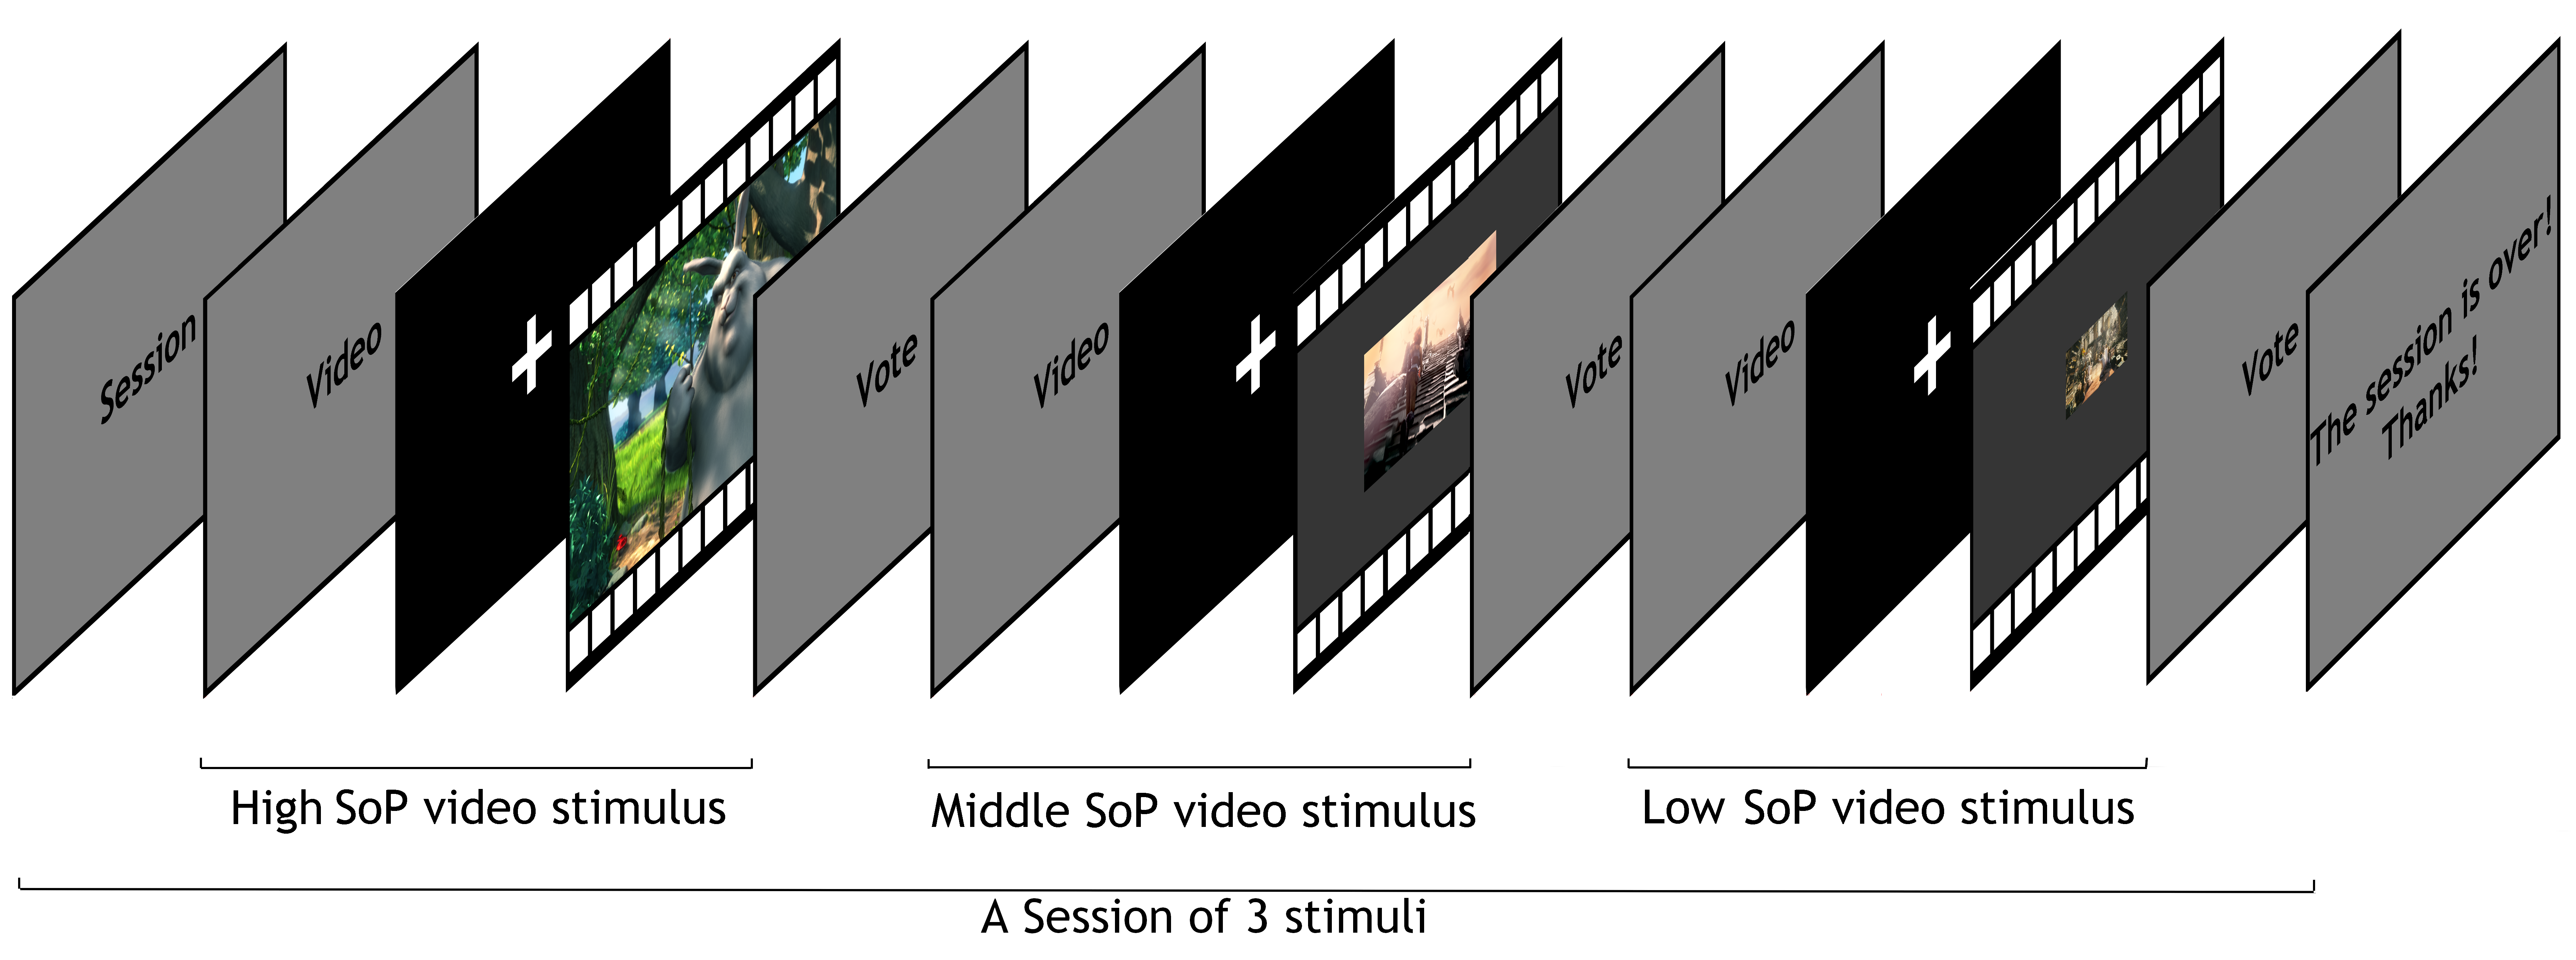
\includegraphics[width=0.5\textwidth]{./images/ExSession_.png}
    \caption{Example of a 3 video stimuli session progress }
    \label{session}
\end{figure}









